\chapter{Introduction}

Computational fluid dynamics (CFD) simulations of blood flow through the
arterial network can take hours to run even on modern hardware, which
makes them impractical for use during a clinical consultation, where a
decision may need to be made within minutes \citep{Diem2017a}.

\section{Motivation}
Reduced-order one-dimensional (1D) blood flow models approximate the full
3D Navier-Stokes equations by averaging over the vessel cross-section,
trading some spatial detail for a very large reduction in computational
cost \citep{Diem2017b}. Prior 1D models have been validated primarily
against idealised geometries rather than patient-specific vessel networks.

\section{Contributions}
This thesis makes the following contributions:
\begin{itemize}
  \item A reduced-order 1D blood flow model validated against full 3D CFD
    simulations across a range of patient-specific vessel geometries.
  \item A comparison against in vivo pressure and flow measurements from
    an existing clinical dataset.
  \item An analysis of the run-time and accuracy trade-off relative to
    full 3D simulation, showing the model is fast enough for real-time
    use at a clinically acceptable accuracy.
\end{itemize}

\begin{figure}
  \center
  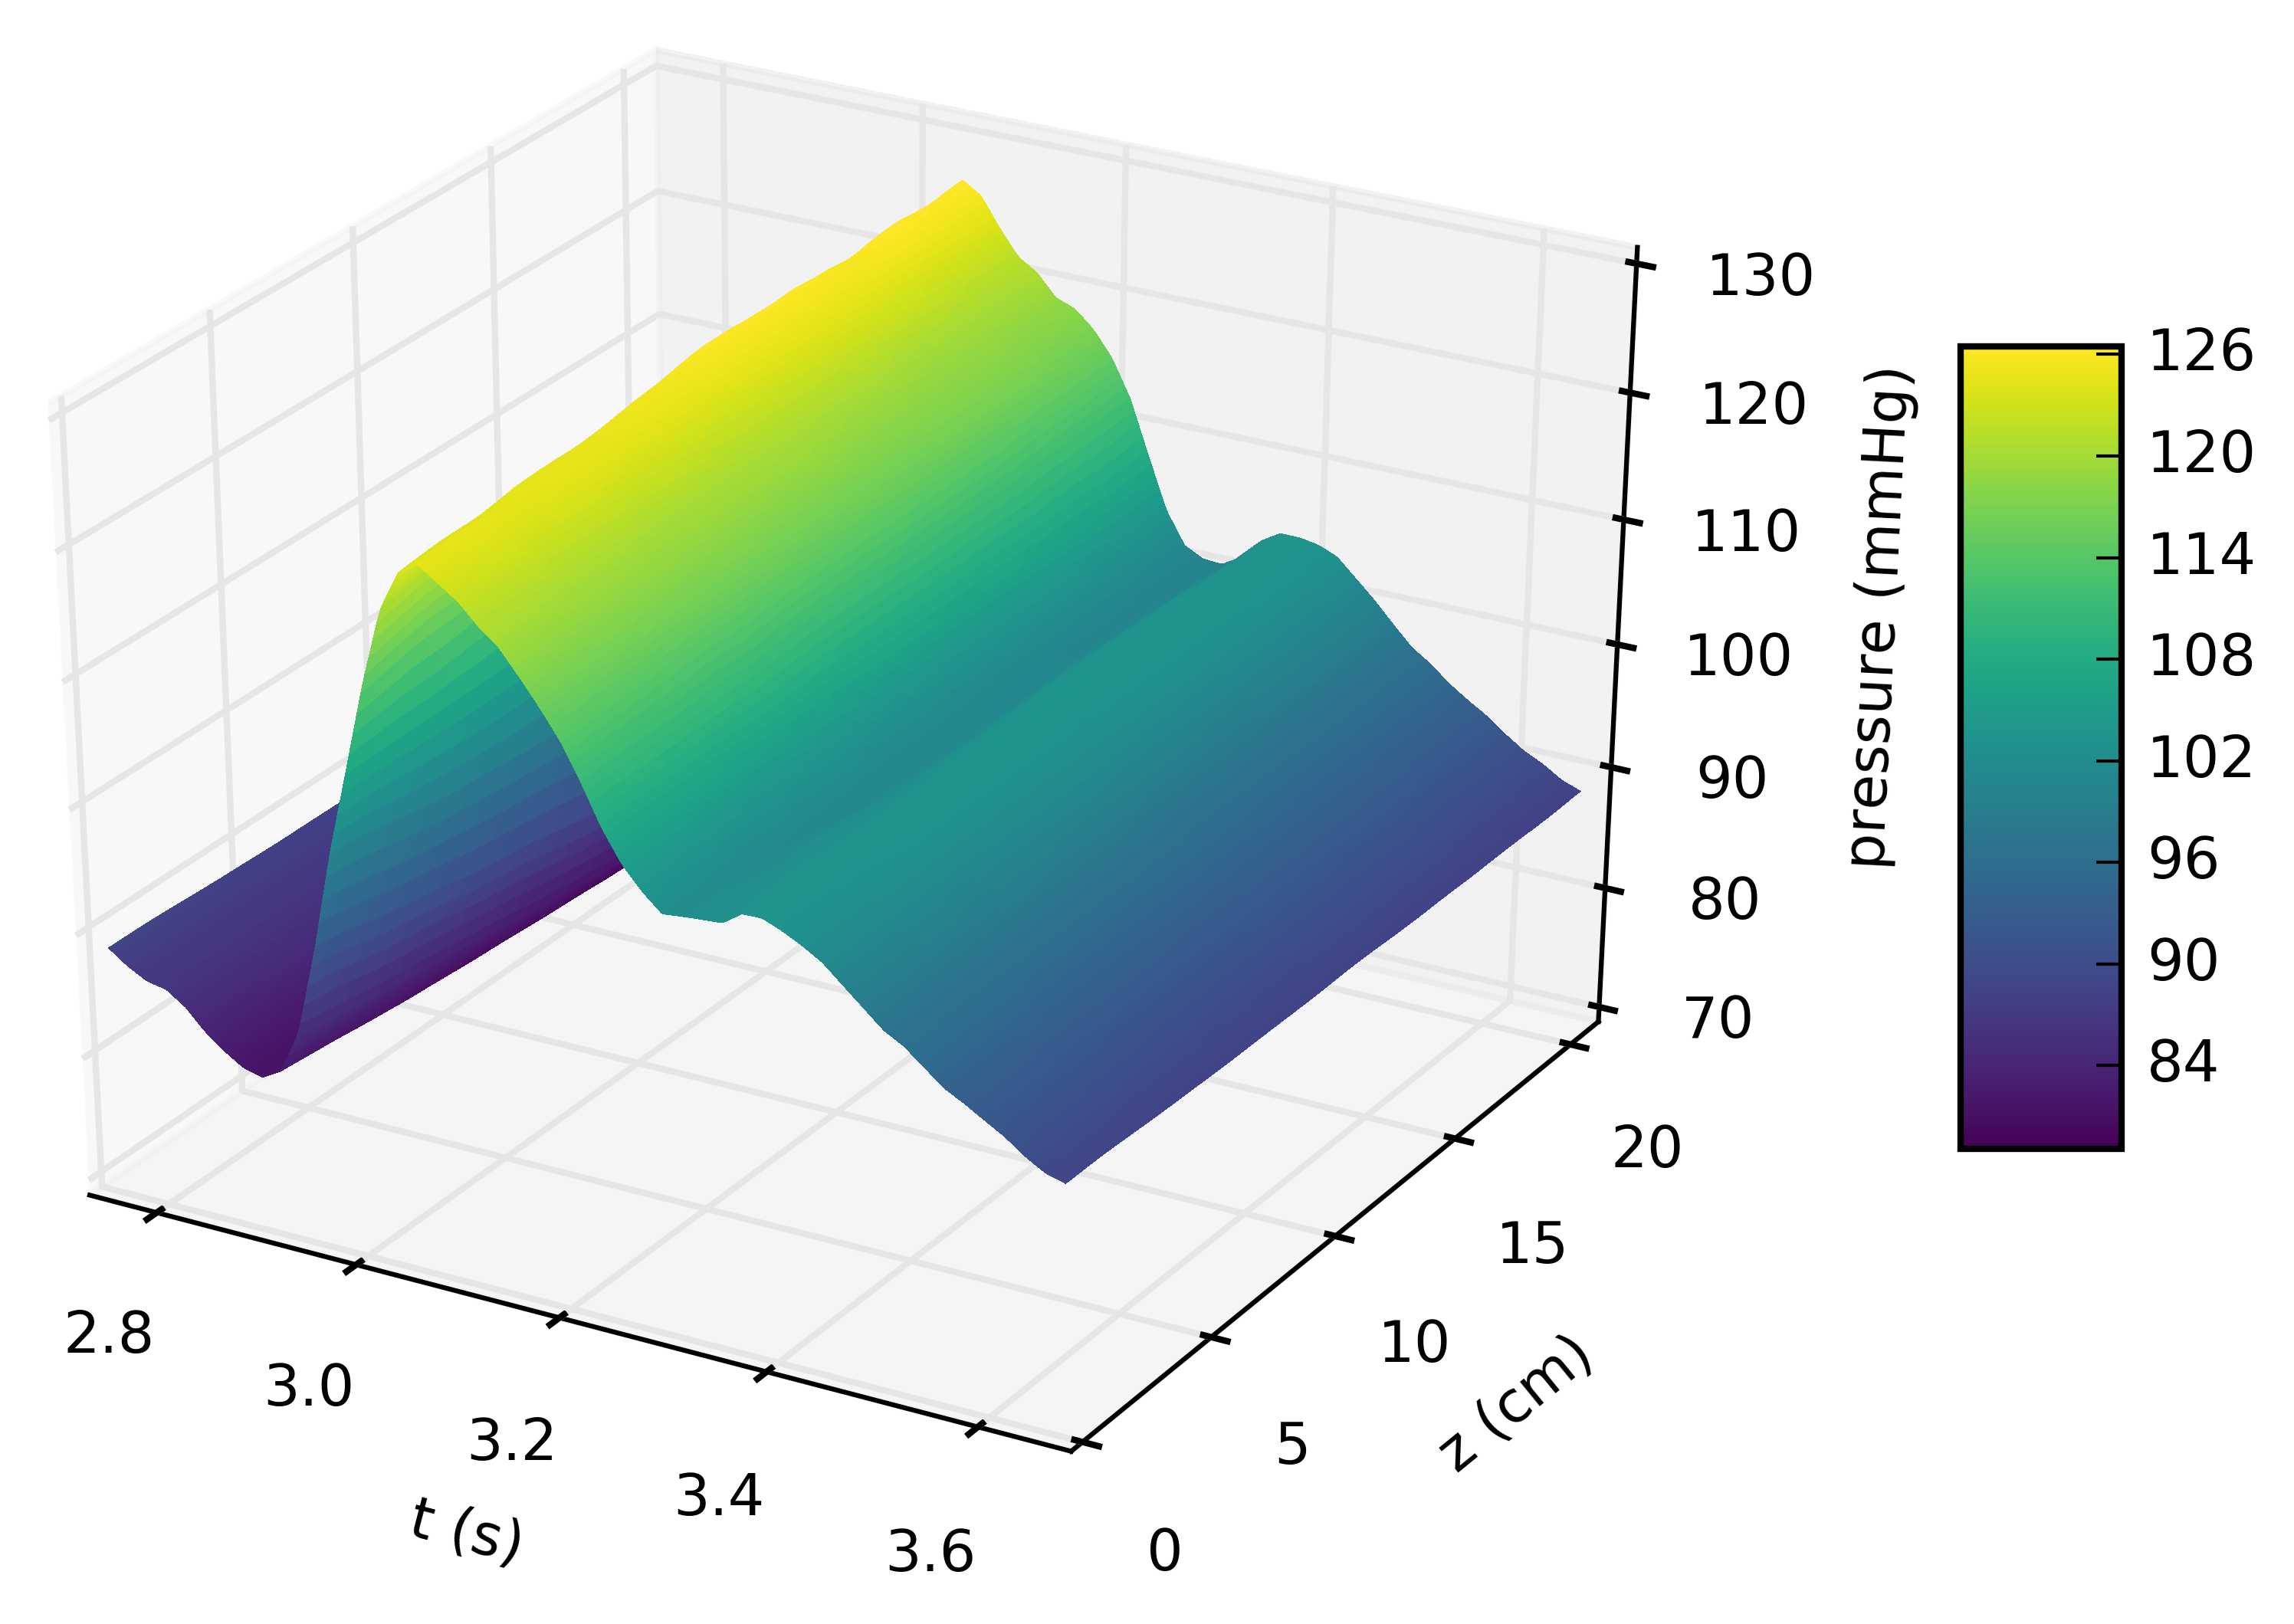
\includegraphics[width=0.6\linewidth]{figure.png}
  \caption{Illustrative one-dimensional discretisation of an arterial segment.\label{fig:1}}
\end{figure}

It references \fref{fig:1}.

\begin{table}
  \center
  \caption{Vessel segments included in the validation dataset.\label{tab:1}}
  \begin{tabular}{cc}
    \toprule
    Segment & Number of Cases\\
    \midrule
    Aorta & 12\\
    Carotid & 9\\
    Femoral & 7\\
    \bottomrule
  \end{tabular}
\end{table}

It also references \tref{tab:1}.
